% Author: Izaak Neutelings (October 2021)
% Description: Rapidity regions of dijet events
% Inspiration:
%  Daniel Savoiu, https://indico.cern.ch/event/1073619/#5-update-on-dijet-production-s
\documentclass[border=3pt,tikz]{standalone}
\usepackage{amsmath}
\usepackage{listofitems} % for \readlist to create arrays
\usepackage{xcolor}
\usepackage[outline]{contour} % glow around text
\usetikzlibrary{calc}
\usetikzlibrary{math} % for \tikzmath
\contourlength{1.0pt}
\tikzset{>=latex} % for LaTeX arrow head

\colorlet{myorange}{orange!80!red!85!black}
\colorlet{mypurple}{blue!50!red}
\colorlet{mygray}{blue!20!black!30}

\newcommand\jetcone[5][blue]{{
  \pgfmathanglebetweenpoints{\pgfpointanchor{#2}{center}}{\pgfpointanchor{#3}{center}}
  \edef\ang{#4/2}
  \edef\e{#5}
  \edef\vang{\pgfmathresult} % angle of vector OV
  \tikzmath{
    coordinate \C;
    \C = (#2)-(#3);
    \x = veclen(\Cx,\Cy)*\e*sin(\ang)^2; % x coordinate P
    \y = tan(\ang)*(veclen(\Cx,\Cy)-\x); % y coordinate P
    \a = veclen(\Cx,\Cy)*sqrt(\e)*sin(\ang); % vertical radius
    \b = veclen(\Cx,\Cy)*tan(\ang)*sqrt(1-\e*sin(\ang)^2); % horizontal radius
    \angb = acos(sqrt(\e)*sin(\ang)); % angle of P in ellipse
  }
  \coordinate (tmpL) at ($(#3)-(\vang:\x pt)+(\vang+90:\y pt)$); % tangency
  \coordinate (tmpO) at ($(#2)+(\vang:0.01)$); % origin shifted
  \coordinate (tmpO') at ($(#2)+(\vang:0.02)$); % origin shifted 2
  \draw[thin,#1!40!black,rotate=\vang, %,fill=#1!50!black!80
    top color=#1!60!black!90,bottom color=#1!70!black!75,shading angle=\vang]
    (#3) ellipse({\a pt} and {\b pt});
  \draw[thin,#1!40!black,rotate=\vang,
  top color=#1!90!black!40,bottom color=#1!40!black!60,shading angle=\vang]
    (tmpL) arc(180-\angb:180+\angb:{\a pt} and {\b pt})
    -- (tmpO) -- cycle;
}}
\def\tick#1#2{\draw[thick] (#1) ++ (#2:0.1) --++ (#2-180:0.2)}


\begin{document}


% DIJET EVENTS
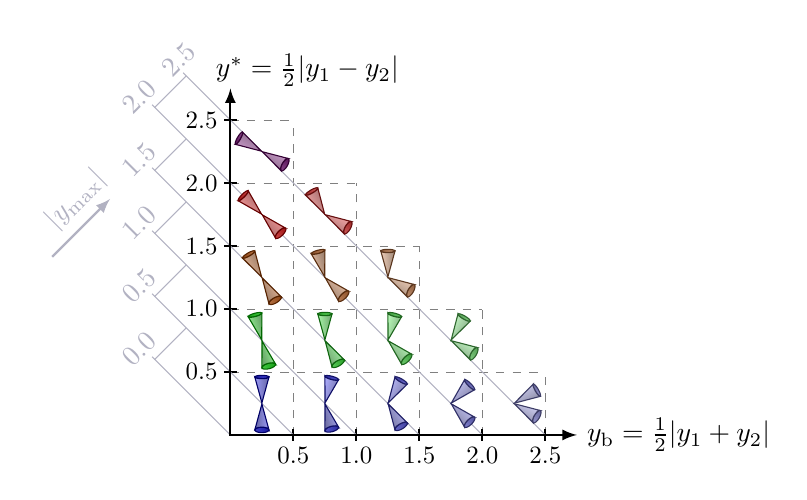
\begin{tikzpicture}[scale=0.8]

  \def\N{5}
  \def\R{1.0}
  \readlist\cols{blue,green,myorange,red,mypurple} % list of colors
  
  % GRIDS
  \foreach \i [evaluate={\y=\i-0.5; \ym=0.5*(\i-1); \Nx=\N-\i+1; \e=0.5*\i}] in {1,...,\N}{
    \draw[very thin,dashed,black!50] (0,\i) --++ (\Nx,0);
    \draw[very thin,dashed,black!50] (\i,0) --++ (0,\Nx);
    \draw[mygray]
      (\i-1,0) --++ (135:{sqrt(2)*(\i+0.2)}) coordinate (T\i) --++ (45:{sqrt(2)/2});
    \draw[mygray] (T\i) --++ (135:0.06) node[above=-2,rotate=45] {\ym};
    \tick{0,\i}{0} node[left=-1,scale=0.9] {\e};
    \tick{\i,0}{90} node[below=-1,scale=0.9] {\e};
  }
  \draw[mygray] (\N,0) --++ (135:{sqrt(2)*(\N+0.75)}) node[right=3,above=0,rotate=45] {2.5};
  
  % JETS
  \foreach \i [evaluate={\y=\i-0.5; \Nx=\N-\i+1; \e=0.5*\i}] in {1,...,\N}{
    \foreach \j [evaluate={\x=\j-0.5; \mix=100-60*(\j-1)/(\N-1);
                           \ang=60*(\i-1)/(\N-1); % seperation
                           \dang=90-60*(\j-1)/(\N-1); % boost
                 }] in {1,...,\Nx}{
      \colorlet{conecol}{\cols[\i]!\mix} % color for cone
      \coordinate (O) at (\x,\y); % primary vertex
      \coordinate (T) at ($(\x,\y)+(\ang+\dang:0.42)$); % top jet
      \coordinate (B) at ($(\x,\y)+(\ang-\dang:0.42)$); % bottom jet
      \jetcone[conecol]{O}{T}{30}{0.06} %!70!white
      \jetcone[conecol]{O}{B}{30}{0.16}
    }
  }
  
  % AXIS
  \draw[<->,thick]
    (0,1.1*\N) %node[left] {\contour{white}{$y*$}} --
    node[left=6,above right=-3] {$y^* = \frac{1}{2}|y_1-y_2|$} --
    (0,0) -- (1.1*\N,0) node[right] {$y_\text{b} = \frac{1}{2}|y_1+y_2|$};
  \draw[->,thick,mygray]
    (135:4.0) --++ (45:1.3)
    node[pos=0.7,above,rotate=45] {$|y_\text{max}|$};
  
\end{tikzpicture}


\end{document}